\documentclass[mathNotesPreamble]{subfiles}
\begin{document}
%\relscale{1.4} %TODO
\section{15.2: Limits and Continuity}

  \begin{defn*}[Limit of a Function of Two Variables]
    The function $f$ has the \textbf{limit} $L$ as $P(x,y)$ approaches $P_0(a,b)$, written
      \[\lim_{(x,y)\to (a,b)} f(x,y)=\lim_{P\to P_0}f(x,y)=L,\]
    if, given any $\eps>0$, there exists a $\delta>0$ such that
      \[\abs{f(x,y)-L}<\eps\]
    whenever $(x,y)$ is in the domain of $f$ and 
      \[0< \abs{PP_0}=\sqrt{(x-a)^2+(y-b)^2}<\delta.\]
  \end{defn*}
  \vspace*{\stretch{1}}
  \textit{Note:} For functions with 1 independent variable, $\abs{x-a}<\delta$ represents an open interval on a number line. Recall that these limits only exist if the same value is approached from two directions.
  
  For functions with 2 independent variables, $\abs{PP_0}<\delta$ represents an open disk (open ball). Here, the limit only exists if the same value is approached from \textit{all} directions.

  \begin{center}
    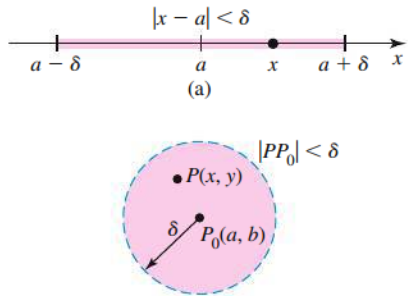
\includegraphics[width=0.5\linewidth]{images/briggs_15_02/fig15_19}
  \end{center}
  \pagebreak

  \begin{thmBox*}[Theorem 15.1: Limits of Constant and Linear Functions]
    Let $a$, $b$, and $c$ be real numbers.
    \begin{enumerate}
      \TabPositions{0.45\linewidth}
      \item Constant function $f(x,y)=c$: \tab $\ds\lim_{(x,y)\to (a,b)} c=c$
      \item Linear function $f(x,y)=x$: \tab $\ds\lim_{(x,y)\to (a,b)} x=a$
      \item Linear function $f(x,y)=y$: \tab $\ds\lim_{(x,y)\to (a,b)} y=b$
    \end{enumerate}
  \end{thmBox*}
  \vspace*{\stretch{1}}

  \begin{thmBox*}[Theorem 15.2: Limit Laws for Functions of Two Variables]
    Let $L$ and $M$ be real numbers and suppose $\ds\lim_{(x,y)\to (a,b)} f(x,y)=L$ and \newline $\ds\lim_{(x,y)\to (a,b)} g(x,y)=M$. Assume $c$ is constant, and $n>0$ is an integer.
    \begin{enumerate}[itemsep=0.65\baselineskip]
      \TabPositions{0.325\linewidth, 0.7\linewidth}
      \item \textbf{Sum} \tab $\ds\lim_{(x,y)\to (a,b)} \parens{f(x,y)+g(x,y)}=L+M$
      \item \textbf{Difference} \tab $\ds\lim_{(x,y)\to (a,b)} \parens{f(x,y)-g(x,y)}=L-M$
      \item \textbf{Constant multiple} \tab $\ds\lim_{(x,y)\to (a,b)} cf(x,y)=cL$
      \item \textbf{Product} \tab $\ds\lim_{(x,y)\to (a,b)} f(x,y)g(x,y)=LM$
      \item \textbf{Quotient} \tab $\ds\lim_{(x,y)\to (a,b)} \frac{f(x,y)}{g(x,y)}=\frac{L}{M}$, \tab provided $M\neq 0$
      \item \textbf{Power} \tab $\ds\lim_{(x,y)\to (a,b)} \parens{f(x,y)}^n=L^n$
      \item \textbf{Root} \tab $\ds\lim_{(x,y)\to (a,b)} \parens{f(x,y)}^{1/n}=L^{1/n}$, \tab when $L>0$ if $n$ is even.
    \end{enumerate}
  \end{thmBox*}
  \pagebreak

  \begin{ex*}
    Evaluate the following limits:
  \end{ex*}

  \begin{tasks}[after-item-skip=\stretch{1}, label=](2)
    \task $\ds\lim_{(x,y)\to (4,11)} 570$
    \task $\ds\lim_{(x,y)\to (2,8)} \parens{3x^2y+\sqrt{xy}}$
    \task $\ds\lim_{(x,y)\to (0,\pi)} \frac{\sin(xy)+\cos(xy)}{7y}$
    \task $\ds\lim_{(x,y)\to (\frac{1}{3},-1)} \frac{9x^2-y}{3x+y}$
  \end{tasks}
  \vspace*{\stretch{1}}
  \pagebreak

  \begin{defn*}[Interior and Boundary Points]
    Let $R$ be a region in $\bbr^2$. An \textbf{interior point} $P$ of $R$ lies entirely within $R$, which means it is possible to find a disk centered at $P$ that contains only points of $R$.
    \vspace*{\baselineskip}
    
    A \textbf{boundary point} $Q$ of $R$ lies on the edge of $R$ in the sense that every disk centered at $Q$ contains at least one point in $R$ and at least one point not in $R$.
  \end{defn*}
  \begin{center}
    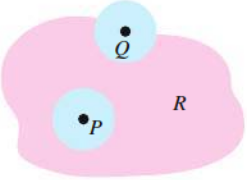
\includegraphics[width=0.25\linewidth]{images/briggs_15_02/fig15_22}
  \end{center}

  \begin{defn*}[Open and Closed Sets]
    A region is \textbf{open} if it consists entirely of interior points. A region is \textbf{closed} if it contains all its boundary points.
  \end{defn*}
  \begin{ex*}
    Identify which regions are open sets and which are closed sets.
  \end{ex*}
  \begin{tasks}[after-item-skip=\stretch{1}, label=](2)
    \task $\set{(x,y): x^2+y^2 < 9}$
    \task $\set{(x,y): \abs{x}\leq 1, \abs{y}\leq 1}$
    \task $\set{(x,y): x\neq 0, -1\leq y\leq 3}$
    \task $\set{(x,y): x+y<2}$
  \end{tasks}
  \vspace*{\stretch{1}}
  \pagebreak

  A limit at a boundary point $P_0(a,b)$ of a function's domain can exist, provided $f(x,y)$ approaches the same value as $(x,y)$ approaches $(a,b)$ \textit{along all paths that lie in the domain}.
  \begin{ex*}
    $\ds f(x,y)=\frac{x^2-y^2}{x-y}$
  \end{ex*}
  \vspace*{\stretch{0.75}}

  \begin{ex*}
    Evaluate the following limits
  \end{ex*}
  \begin{tasks}[after-item-skip=\stretch{1}, label=](2)
    \task $\ds\lim_{(x,y)\to (0,\pi)} \frac{\sin(xy)+\cos(xy)}{7y}$
    \task $\ds\lim_{(x,y)\to (-3,-15)} \frac{y^2-5xy}{y-5x}$
    \task $\ds\lim_{(x,y)\to (0,0)} \frac{x+2y}{x-2y}$
    \task $\ds\lim_{(x,y)\to (1,-1)} \frac{y^5}{(x-1)^{30}+y^5}$
  \end{tasks}
  \vspace*{\stretch{1}}

  \begin{thmBox*}[Procedure: Two-Path Test for Nonexistence of Limits]
    If $f(x,y)$ approaches two different values as $(x,y)$ approaches $(a,b)$ along two different paths in the domain of $f$, then $\ds\lim_{(x,y)\to (a,b)} f(x,y)$ does not exist.
  \end{thmBox*}
  \pagebreak

  \begin{defn*}[Continuity]
    The function $f$ is continuous at the point $(a,b)$ provided
    \begin{enumerate}
      \item $f$ is defined at $(a,b)$
      \item $\ds\lim_{(x,y)\to (a,b)} f(x,y)$ exists, and 
      \item $\ds\lim_{(x,y)\to (a,b)} f(x,y) = f(a,b)$.
    \end{enumerate}
  \end{defn*}

  \begin{ex*}
    Determine if $f(x,y)$ is continuous at $(0,0)$
      \[f(x,y)=\begin{cases}
        \ds\frac{3xy^2}{x^2+y^4}, &\textnormal{if } (x,y)\neq (0,0)\\
        0, &\textnormal{if } (x,y)=(0,0)
      \end{cases}\]
  \end{ex*}
  \vspace*{\stretch{1}}

  \begin{thmBox*}[Theorem 15.3: Continuity of Composite Functions]
    If $u=g(x,y)$ is continuous at $(a,b)$ and $z=f(u)$ is continuous at $g(a,b)$, then the composite function $z=f\parens{g(x,y)}$ is continuous at $(a,b)$.
  \end{thmBox*}

  \begin{ex*}
    Determine the points at which the following functions are continous:
  \end{ex*}
  \begin{tasks}[after-item-skip=\stretch{1}, label=](2)
    \task $f(x,y)=\ln(x^2+y^2+4)$
    \task $g(x,y)=e^{x/y}$
  \end{tasks}
  \vspace*{\stretch{1}}
  \pagebreak

\end{document}